\subsubsection{,,DiseaseCore" pakotne}
\subsubsection*{Multithreading}
Darba autors jau projekta plānošanas stadijā zināja, ka vēlēsies padziļināti
izpētīt un apgūt \emph{multithreaded} aplikācijas izstrādes principus, tāpēc jau pašā sākumā
centās saprast, kur projektā varētu veidot paralēlo darbību.

Šāda nepieciešamība noveda pie sekojošās koda arhitektūras, kuras vispārīgo
vizuālo reprezentāciju var apskatīt \ref{img:multithreaded-layout} attēlā: visa plakne, kur tiks
veikta simulācija, tiek sadalīta vienādos reģionos pa \(x\) asi (kods -- \emph{Region.cs} fails).
Katrā reģionā atrodas kaut kāda noteiktu sākotnējo entītiju (gan veselo, gan slimo) apakškopa,
tie tiek ievietoti savā reģionā no to attiecīgajām \(x\) ass koordinātām.

Katrs reģions tiek piešķirts noteiktai \emph{Task}\cite{csharp:task} instancei.
Tajā brīdī, kad noteiktā entītija šķērso \emph{Region} \(x\)ass robežas, tad tā tiek
ievietota \emph{Out of bounds} buferī (kopīgs visām \emph{Region} instancēm), kuru
regulāri apstrādā cita \emph{Task} instance - katra entītija šajā \emph{Out of bounds} buferī tiek
izvērtēta pēc tās atrašanās vietas (pa \(x\) asi) un tiek novietos attiecīgā \emph{Region}
\emph{inbound} buferī, kuru brīvā brīdī noteiktā \emph{Region} pārvaldošais \emph{Task} pievienos
simulējamajām entītijām. Šo entītiju kārtošanas kodu var apskatīt
\ref{app:out-of-bounds-sorting} pielikumā.


\begin{figure}[H]
	\centering
	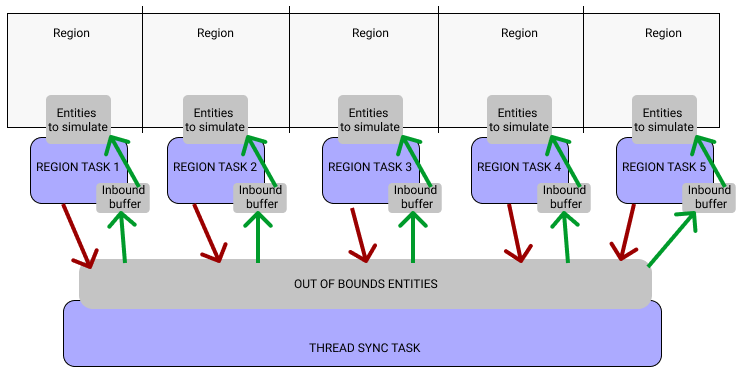
\includegraphics[scale=0.5]{images/multithreaded-layout.png}
	\caption{Reģionu sadalījums plaknei}
	\label{img:multithreaded-layout}
\end{figure}

Nepieciešamība izveidot \emph{inbound} buferi priekš \emph{Region} radās tādēļ, lai
nerastos situācija,
ka entītiju simulācijas brīdī (kur tiek veikta iterēšana pār entītijām iekš \emph{Region}) pēkšņi
rastos kaut kādas modifikācijas no cita \emph{thread} -- \emph{data races}.

Izvēle dalīt visu simulācijas laukumu reģionos pa \(x\) asi (varēja būt arī \(y\)
ass, tikai ne abas asis reizē), bija tāpēc, lai ērti varētu to pielāgot dažādu
kodolu skaitam, ko var ērti realizet, ja plakne tiek dalīta tikai pa vienu asi.

Darba autors \textbf{neizmanto visus pieejamos procesora kodolus priekš \emph{Region} pārvaldības}, jo šādā gadījumā
procesors tiek pārslogots un tiek kavēta \emph{UI} atjaunošanās (par to
vēlāk tiks aprakstīts), tāpēc tiek izmantota tikai \(\frac{2}{3}\) no
pieejamajiem procesora kodoliem (vai sliktākajā gadījumā 1 kodols). Šī iemesla dēļ
\ref{img:multithreaded-layout} attēlā ir parādīti 5 reģioni/5 \emph{Tasks}/ \(\frac{2}{3}\) no 8 kodolu sistēmas.

Lai gan, ņemot vērā, ka \(1 Task\neq 1 Thread\), jo \emph{Taski} izpildās uz \emph{.NET Runtime}
pieejama \emph{threadpoola}\cite{csharp:tasks-not-threads}, tad reāli definēt vairāk
\emph{Tasks} arī ir iespējams -- \emph{runtime} definētie \emph{threadi} (mēdz saukt arī par
\emph{green threads}\cite{progr:green-threads}) izpildās
sistēmas \emph{userspace}\cite{sys:userspace}, nevis sistēmas \emph{kerneļa} līmenī, kas \emph{.NET Runtime}
atļauj pašam izlemt, kad darīt \emph{vienlaicīgas vai paralēlas}\cite{csharp:concurrent-parallel} darbības.
\emph{Tasku} pārvaldība iekš
\emph{userspace} ar esošu \emph{threadpool} ir daudz ātrāka nekā zemā līmeņa \emph{kernel thread} veidošana
katram izsaukumam.

Visi \emph{Task} dalītie resursi tiek ,,aizsargāti" ar \emph{Mutex}\cite{csharp:mutex}
instancēm, kas garantē to, ka informācija (aizsargātais mainīgais) netiks vienlaicīgi lasīts/rakstīts no
vairākiem citiem \emph{threadiem} vienlaicīgi -- datu integritāte tiek saglabāta. Izstrādes procesā
pareiza \emph{Mutex} implementācija radīja daudzas kļūdas -- \emph{data races} un \emph{deadlocks}.

% CHAPTER LINQ un Pipeline
\subsubsection*{Pipeline}

Lai sistēmā varētu nodrošināt funkciju modularitāti -- karantīna slimajiem,
definēti kopīgie saskarsmes punkti, \emph{zombie mode}, utt. -- bija nepieciešams
izplānot kādā veidā šo funkcionalitāti varētu ieslēgt un izslēgt koda izpildes
laikā. Darba autors izvēlējās funkciju kompozīcijas dizaina modeli --
\emph{Pipelines}\cite{progr:pipelines}. Pirms tiek izveidota galvenā simulācijas
instance \emph{World}(fails \emph{World.cs}), ir jāinicializē \emph{List} ar
\emph{Pipeline} (fails \emph{BasePipeline.cs}, skat. \ref{app:IPipeline} pielikumā)
interfeisa implementējošām instancēm.

Tips \emph{PipelineReturnData}, kuru atgriež \emph{pushThrough} funkcija \ref{app:IPipeline} pielikumā, ir
uzskatāms par \emph{type alias} \emph{Tuple<T, K>} mainīgajam:

{
\setstretch{1}
\begin{minted}{CSharp}
(List<EntityOnMap<SickEntity>>, List<EntityOnMap<HealthyEntity>>)
\end{minted}
}

, jo \emph{C\#} nepiedāvā valodas konstrukciju, kas atļautu definēt
\emph{type alias} priekš dažādām esošām koda struktūrām. Šajā gadījumā tas tika
darīts ar jaunas klases palīdzību, lai kods būtu lasāmāks.

Tālāk ir jāveido klases, kas implementē šo \emph{Pipeline} interfeisu -- katrai sistēmas
nepieciešamajai darbībai jāveido sava klases ar interfeisa implementāciju. Kopā
tika izveidoti 8 dažādi \emph{pipeline} objekti:

\begin{enumerate}
    \item \textbf{AttractorPipeline} -- definē rutīnas entītijām, vietas uz kuriem visas kopīgi dosies.
    \item \textbf{DeathPipeline} -- izņem entītiju no saraksta, ja tā dzīvības ir vienādas ar \(0\).
    \item \textbf{GeoLocationPipeline} -- pārvieto entītiju kartē, aprēķinot tās jauno
        atrašanās vietu, zinot entītijas virzienu, ātrumu, esošo lokāciju un pagājušo
        laiku kopš iepriekšējās iterācijas.
    \item \textbf{InfectionPipeline} -- pārbauda, kuras veselās entītijas ir blakus slimajam
        entītijām un konvertē tos uz slimajām entītijām.
    \item \textbf{QuarantinePipeline} -- visas slimās entītijas novieto noteiktā plaknes
        stūrī, lai izslimotu savu slimību.
    \item \textbf{RecoveryPipeline} -- ja slimā entītija ir atveseļojies, tad konvertē to uz veselo entītiju.
    \item \textbf{TickingPipeline} -- iedarbina entītijas ,,iekšējo" pulksteni (pārrēķina jaunu kustības virzienu, veselības stāvokli).
    \item \textbf{ZombieModePipeline} -- liek visām slimajām entītijām virzīties pretī vistuvākajam veselajām entītijām.
    \item \textbf{AssertionPipeline} -- \emph{runtime} pārbaude vai visas entīijas tipi ir
        pareizi sadalīti (iepriekš tika izmantota dinamisku datu tipu
        pārvēršana (\emph{type casting}) \emph{runtime} laikā, tāpēc šis \emph{pipeline} bija
        noderīgs priekš kļūdu izķeršanas, bet šobrīd tā darbības jēga ir zudusi).
\end{enumerate}

Dažādie \emph{Pipeline}, kur tiek veiktas starp-entītiju pārbaudes, notiek tikai
katra \emph{Region} iekšējās robežās -- tas ir efektīvi sistēmai, bet \emph{Region}
dalījums par \(x\) asi dažreiz mēdz ierobežot entītiju uzvedību.

Sistēmas izstrādes laikā ir jāpievērš uzmanība arī \emph{pipeline} secībai, jo katrs \emph{pipeline}
operē ar iepriekšējā pipeline modificētajiem datiem -- izmainot secību
(vai arī izslēdzot/ieslēdzot kādu \emph{pipeline}) var rasties atšķirīgi iznākumi.

Katrai sistēmas \emph{Region} instancei ir pieejams inicializētais \emph{List<Pipeline>}
objekts, tad ar \emph{LINQ} palīdzību \emph{Region} izpildes ciklā tā iekšējos entītijus
,,izlaiž" cauri \emph{pipeline} sarakstam (\emph{Region.cs} failā, skat. \ref{app:pipelien-linq} pielikumā):

Papildus uzsvars uz \emph{LINQ} izmantošanu šajā kursa darba atskaitē nebūs veikts,
jo tas tika izmantots pilnībā visās \emph{Pipeline} implementācijās, gandrīz vai
visās simulācijas funkcijas un pat \emph{UI} saskarnē. Tika izmantotas dažādas šis
funkcionālas paradigmas metodes vairākās vietās kodā -- \emph{Aggregate, Where, Select, Concat, Min, Max, u.c.}.


\subsubsection{,,frontendserver" pakotne}

% Blazor UI kontrolē pipelines un instanciēšanu

Lietotāju saskarne ir programmēta ar \emph{Blazor Server} ietvaru. Sākotnēji darba
autors vēlējas izmantot \emph{Blazor WebAssembly} \emph{dotnet template} versiju,
lai varētu visu projektu novietot kā \emph{SPA}\cite{progr:SPA} uz statiskā faila servera. Tomēr
pašreizējā \emph{Blazor} versija nepiedāvā vairāku procesu paralelizācijas iespējas
(tikai \emph{concurrent} iespējamību, izmantojot vienu \emph{threadu}, kas arī ir
izmantots priekš pārlūkprogrammas \emph{UI} zīmēšanas)\cite{csharp:blazor-no-multithreaded-support}. Lai gan
visi \emph{WEB} brosweri kopš 2020. gada vasaras atbalsta \emph{WebAssembly Threads}
priekšlikumu \cite{wasm:threads-proposal}, tomēr to ir nepieciešams atsevišķi
,,ieslēgt" caur pārlūkprogrammas iestatījumiem. Otrs veids kā iegūt paralelizāciju \emph{WEB}
lietojumprogrammas ir ar \emph{WebWorkers}, bet lai to paveiktu, ir nepieciešama
papildus \emph{JavaScript} ,,līme".

\emph{Blazor WebAssembly} neatbalsta nevienu variantu vairāku
sistēmas \emph{threadu} izveidei. Šī iemesla dēļ tika izmantots \emph{Blazor Server}
versija, kur visa \emph{UI} apstrāde (arī simulācijas palaišana) notiek \textbf{uz servera}. Šāda
pieeja gan nozīmē, to, ka reāli uz serveriem publiskai pieejai šo sistēmu novietot nav laba doma -- jo
vairāk cilvēki pieslēgsies un veiks simulācijas, jo lielāka slodze un sliktāk tā strādās.
Tomēr tā ir problēma ārpus šī kursa darba ietvariem.

% Canvas pakotne
Pati attēla zīmēšana tiek veikta uz \emph{HTML5 Canvas} elementa\cite{html5:canvas}.
Šis elements piedāvā \emph{JavaScript API}, lai zīmētu reāla laika grafikas, attēlus, animācijas.
Tiek piedāvāti dažādi \emph{API} paveidi kā zīmēt lietas -- ,,2d", ,,webgl", ,,webgl2",
,,bitmaprenderer" \cite{html5:canvas-contexts}. Tomēr šie ir \emph{JavaScript API}, lai
no \emph{C\#} tos izsauktu, ir nepieciešams izveidot \emph{wrapper} funkcijas šim \emph{JS API},
nodrošinot starp-valodu komunikāciju. Darba autoram izdevās atrast jau izveidotu \emph{Blazor} bibliotēku,
kas nodrošina šo \emph{JavaScript API wrapper} priekš  \emph{HTML5 Canvas} -- \emph{BlazorExtensions.Canvas}
(\url{https://github.com/BlazorExtensions/Canvas}).
Darba autors jau iepriekš bija darbojies ar WebGL, kas nodrošinātu ātru un efektīvu
zīmējuma veidošanu un atjaunināšanu, tomēr šī \emph{BlazorExtensions.Canvas} bibliotēkas
dokumentācijā aprakstītais WebGL piemērs nestrādāja -- tāpēc darba izstrādē tika
izmantots ,,2d" \emph{context API}.

% Data polling
Inicializējot un uzstartējot simulāciju (skat. \ref{app:init-simulation} pielikumā), tā darbojas atsevišķā
sistēmas \emph{threadā} no \emph{UI} saskarnes -- no lietotāju saskarnes puses nav
viens konkrēts moments, kad
varētu iegūt visas nepieciešamās vērtības par esošajām entītijām sistēmā. Risinājums
ir izmantot tādu kā \emph{data polling}\cite{progr:data-polling} pieeju. Paša \emph{Blazor} koda \emph{polling}
pieeja ir apskatāma \ref{app:polling} pielikumā, bet simulācijas atbildi uz šo
vaicājumu var apskatīt \ref{app:polling-world} pielikumā. Koda secību
diagrammu priekš izveidotās \ref{app:polling-world} pielikuma metodes ir iespējams
aplūkot \ref{img:squance-diagram-get-status}
attēlā. Katrā
datu pieprasījuma reizē ir nepieciešams nopauzēt (iekšējais mainīgais, kas raksturo esošo stāvokli) visas \emph{Region} instances,
lai nenotiktu \emph{data races}, nepieciešams pauzēt pašu \emph{World} instanci (lai
\emph{OutOfBounds} sinhronizācija \textbf{nenotiktu} datu nolases brīdī), tad nepieciešams apkopot
datus no visām datu krātuvēm, atpauzēt visas instances, atgriezt datus lietotāju saskarnei.

\begin{figure}[H]
	\centering
	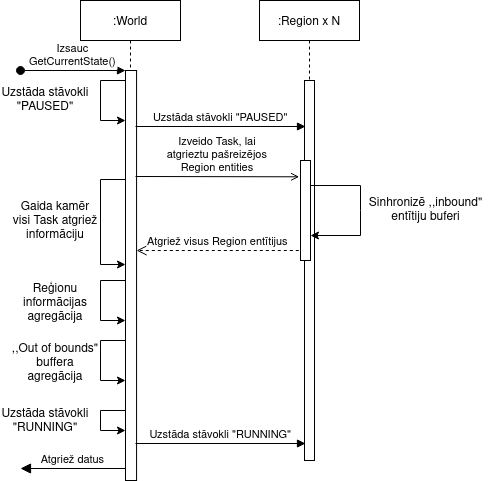
\includegraphics[scale=0.7]{images/DiseaseCore-GetData.png}
	\caption{Simulācijas datu stāvokļa vaicājuma izpilde}
	\label{img:squance-diagram-get-status}
\end{figure}

Tālāk šie iegūtie dati \emph{Blazor} pusē tiek papildus sadalīti: metadati tiek nodoti
\emph{Statistics} komponentei, kas aprēķina katra \emph{Region} ātrdarbību, bet
reāli dati par entītiju stāvokļiem tiek nodota \emph{Canvas} komponentei, kur
entītijas tiek sašķirotas un katra uzzīmēta uz \emph{HTML canvas} ar \emph{BlazorExtensions.Canvas} bibliotēkas palīdzību.
